\documentclass[a4paper,12pt]{letter}

\usepackage{tikz}
\usepackage{amsmath}
\usepackage{amssymb}
\usepackage{nopageno}
\usepackage[a4paper, total={7.5in, 11.25in}]{geometry}
\usepackage[utf8]{inputenc}
\usepackage[T1]{fontenc}
\usepackage{lmodern}
\usepackage{setspace}
\setstretch{1.2}
\usepackage{pgfplots}
\pgfplotsset{compat=1.18}

\usetikzlibrary{
calc,
3d,
decorations.pathmorphing,
decorations.pathreplacing,
decorations.markings,
snakes,
arrows.meta,
patterns
}

\tikzset{snake it/.style={decorate, decoration=snake}}

\begin{document}

\begin{center}
(KTXFI1EBNF) Physics I. Homework No.~3 Solutions\\[0.2cm]
April~27,~2026
\end{center}

\bigskip

\begin{enumerate}

% =========================================================================================

\item Determine the acceleration of a proton $m = 1.67\cdot10^{-27}\,\mathrm{kg}$ in an electric field of strength $E = 100\,\mathrm{N/C}$. How many times greater is this acceleration than the acceleration due to gravity?

\begin{center}
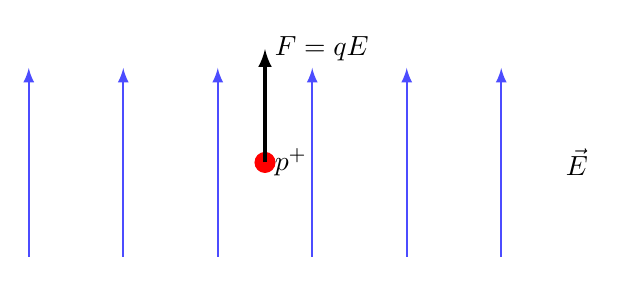
\begin{tikzpicture}[scale=1.2,>=latex]

% Electric field lines
\foreach \x in {0,1,...,5}
{
\draw[->,blue!70,thick] (\x,0) -- (\x,2);
}

% Proton
\filldraw[red] (2.5,1) circle (3pt);
\node[right] at (2.5,1) {$p^+$};

% Force
\draw[->,very thick] (2.5,1) -- (2.5,2.2);
\node[right] at (2.5,2.2) {$F=qE$};

\node at (5.8,1) {$\vec E$};

\end{tikzpicture}
\end{center}
  

The electric force acting on the proton is

$$F=qE.$$

Since the proton charge is

$$q=e=1.602\cdot10^{-19}\,\mathrm{C},$$

its acceleration is

$$a=\frac{F}{m}=\frac{eE}{m}.$$

Substituting the numerical values,

$$a=\frac{(1.602\cdot10^{-19}\,\mathrm{C})(100\,\mathrm{N/C})}{1.67\cdot10^{-27}\,\mathrm{kg}}=9.59\cdot10^9\,\mathrm{m/s^2}.$$

Now compare this with the gravitational acceleration:

$$\frac{a}{g}=
\frac{9.59\cdot10^9\,\mathrm{m/s^2}}{9.81\,\mathrm{m/s^2}}=9.78\cdot10^8.$$

Therefore,

$$\boxed{a=9.59\cdot10^9\,\mathrm{m/s^2}}$$

and the acceleration is approximately

$$\boxed{9.78\cdot10^8}$$

times greater than the acceleration due to gravity.


% =========================================================================================

\newpage
\item An electron is launched with an initial velocity of $v_0 = 2\cdot10^6\,\mathrm{m/s}$ between two parallel charged plates. If the electric field strength between the plates is $E = 2\,\mathrm{kN/C}$, where does the electron hit the upper plate? Assume vacuum.

\begin{center}
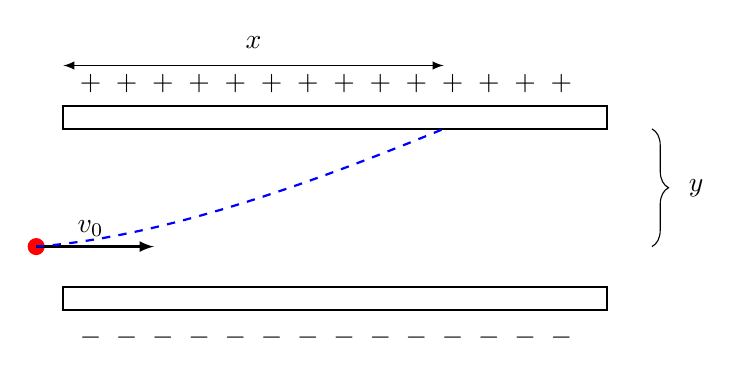
\begin{tikzpicture}[scale=1.15, >=latex]

% Plates
\draw[thick] (0,0) rectangle (6,0.25);
\draw[thick] (0,-2) rectangle (6,-1.75);

% Charges
\foreach \x in {0.3,0.7,...,5.8}
{
\node at (\x,0.5) {$+$};
\node at (\x,-2.3) {$-$};
}

% Electron
\filldraw[red] (-0.3,-1.3) circle (2.5pt);

% Initial velocity
\draw[->,thick] (-0.3,-1.3) -- (1,-1.3);
\node[above] at (0.3,-1.3) {$v_0$};

% Trajectory
\draw[thick,dashed,blue]
(-0.3,-1.3)
.. controls (1,-1.2) and (2.5,-0.7)
.. (4.2,0);

% x arrow
\draw[<->] (0,0.7) -- (4.2,0.7);
\node at (2.1,0.95) {$x$};

% y brace
\draw[decorate,decoration={brace,mirror,amplitude=6pt}]
(6.5,-1.3) -- (6.5,0);
\node[right] at (6.8,-0.65) {$y$};

\end{tikzpicture}
\end{center}

The magnitude of the electric force is

$$F=eE.$$

Thus the vertical acceleration of the electron is

$$a=\frac{eE}{m_e}.$$

Using

$$m_e=9.11\cdot10^{-31}\,\mathrm{kg},$$

we obtain

$$a=\frac{(1.602\cdot10^{-19}\,\mathrm{C})(2000\,\mathrm{N/C})}{9.11\cdot10^{-31}\,\mathrm{kg}}=3.52\cdot10^{14}\,\mathrm{m/s^2}.$$

The vertical motion is uniformly accelerated:

$$y=\frac12 at^2.$$

Therefore,

$$t=\sqrt{\frac{2y}{a}}.$$

The horizontal motion is uniform:

$$x=v_0 t.$$

Hence,

$$x=v_0\sqrt{\frac{2y}{a}}.$$

Substituting the expression for the acceleration:

$$x=v_0\sqrt{\frac{2m_e y}{eE}}.$$

Now substitute the numerical values:

$$x=v_0\sqrt{\frac{2m_e y}{eE}}=2\cdot10^6\sqrt{\frac{2(9.11\cdot10^{-31})y}{(1.602\cdot10^{-19})(2000)\,\mathrm{N/C}}}.$$

This gives

$$\boxed{x=0.151\sqrt{y}},$$

where both \(x\) and \(y\) are measured in meters.

% =========================================================================================

%\newpage
\item An electron enters the region between the plates halfway between them. The plate length is $l=10\,\mathrm{cm},$ their separation is $d=1\,\mathrm{cm},$ and the voltage difference is $U=200\,\mathrm{V}.$ Determine the initial velocity needed for the electron to just barely leave the region between the plates.

\begin{center}
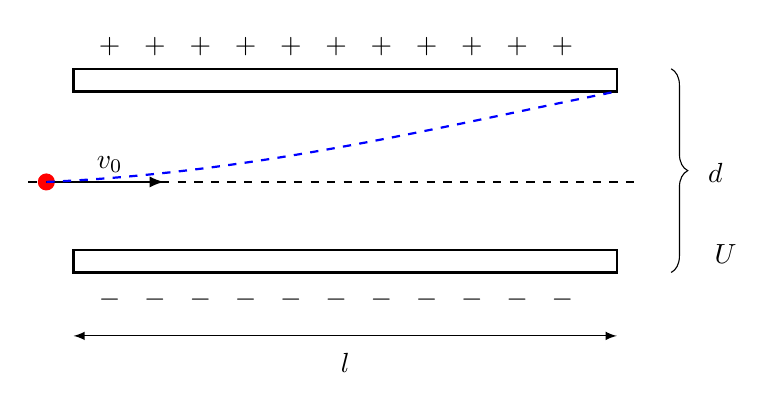
\begin{tikzpicture}[scale=1.15,>=latex]

% Parameters
\def\L{6}
\def\d{2}

% Plates
\draw[thick] (0,0) rectangle (\L,0.25);
\draw[thick] (0,-\d) rectangle (\L,-\d+0.25);

% Charges
\foreach \x in {0.4,0.9,...,5.8}
{
\node at (\x,0.5) {$+$};
\node at (\x,-2.3) {$-$};
}

% Midline
\draw[dashed] (-0.5,-1) -- (\L+0.2,-1);

% Electron
\filldraw[red] (-0.3,-1) circle (2.5pt);

% Velocity
\draw[->,thick] (-0.3,-1) -- (1,-1);
\node[above] at (0.4,-1) {$v_0$};

% Trajectory
\draw[thick,dashed,blue]
(-0.3,-1)
.. controls (2,-0.9) and (4,-0.4)
.. (6,0);

% l arrow
\draw[<->] (0,-2.7) -- (6,-2.7);
\node at (3,-3.0) {$l$};

% d brace
\draw[decorate,decoration={brace,mirror,amplitude=6pt}]
(6.6,-2) -- (6.6,0.25);

\node[right] at (6.9,-0.9) {$d$};

% Voltage
\node at (7.2,-1.8) {$U$};

\end{tikzpicture}
\end{center}


The electric field between the plates is

$$E=\frac{U}{d}.$$

Thus,

$$E=\frac{200\,\mathrm{V}}{0.010\,\mathrm{m}}=2.0\cdot10^4\,\mathrm{N/C}.$$

The electron acceleration is

$$a=\frac{eE}{m_e}=\frac{eU}{m_e d}.$$

Substituting the numerical values,

$$a=\frac{(1.602\cdot10^{-19}\,\mathrm{C})(200\,\mathrm{V})}{(9.11\cdot10^{-31}\,\mathrm{kg})(0.010\,\mathrm{m})}=3.52\cdot10^{15}\,\mathrm{m/s^2}.$$

The electron starts halfway between the plates, therefore its required vertical displacement is

$$\Delta y=\frac{d}{2}.$$

The vertical motion is

$$\frac{d}{2}=\frac12 at^2.$$

Hence,
$$d=at^2,$$

thus,
$$t=\sqrt{\frac{d}{a}}.$$

The horizontal motion is uniform:

$$l=v_0 t.$$

\pagebreak
Therefore,

$$v_0=\frac{l}{t}=l\sqrt{\frac{a}{d}}.$$

Substituting

$$a=\frac{eU}{m_e d},$$

we get

$$v_0=l\sqrt{\frac{eU}{m_e d^2}}.$$

Substituting the numerical values,

$$v_0=l\sqrt{\frac{eU}{m_e d^2}}=0.10\sqrt{\frac{(1.602\cdot10^{-19}\,\mathrm{C})(200\,\mathrm{V})}{(9.11\cdot10^{-31}\,\mathrm{kg})(0.010\,\mathrm{m})^2}}=5.93\cdot10^7\,\mathrm{m/s}.$$

Therefore,

$$\boxed{v_0=5.93\cdot10^7\,\mathrm{m/s}}$$

is required.

\bigskip


\end{enumerate}

\bigskip

\rightline{Dr.~Gabor~FACSKO}
\rightline{\textit{facsko.gabor@uni-obuda.hu}}

\vfill

\end{document}


